\documentclass[12pt, a4paper]{report}
\usepackage{pgf}
\usepackage{tikz}
\usetikzlibrary{automata,arrows}

\title{Homework 1}
\author{Chang Wang}
\date{} % delete this line to display the current date

\begin{document}

\maketitle

For the given program and its parallelism profile. Find the best architecture configuration to run the program with the minimum number of cycles. The best architecture should be defined with the number and particular issues. \\[0.2cm]
What is the best number of cycles for your best architecture. \\[0.5cm]

The software profile for given program looks like below: \\[0.5cm]
\begin{center}
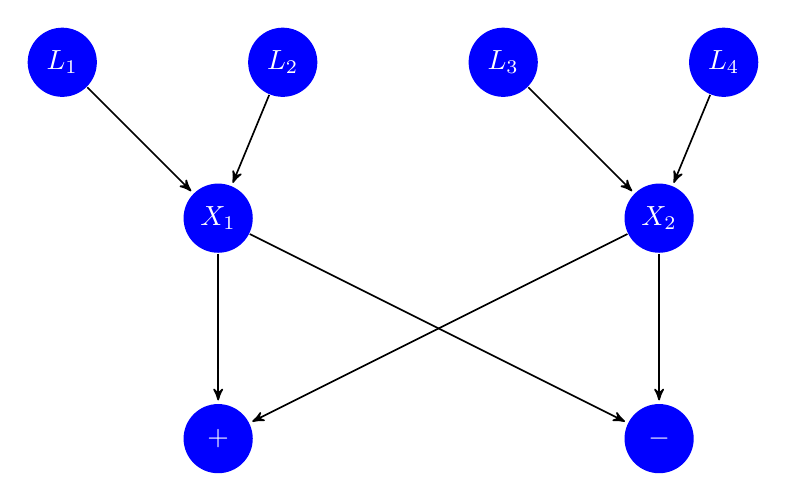
\begin{tikzpicture} 
	[->,>=stealth',shorten >=1pt,auto,node distance=2.8cm, semithick]
	\tikzstyle{every state}=[fill=blue,draw=none,text=white]

	\node[state] (L1)                    {$L_{1}$};
  	\node[state] (L2)  [right of=L1]     {$L_{2}$};
	\node[state] (L3)  [right of=L2]     {$L_{3}$};
	\node[state] (L4)  [right of=L3]     {$L_{4}$};
	\node[state] (X1) [below right of=L1] {$X_{1}$};
	\node[state] (X2) [below right of=L3] {$X_{2}$};
	\node[state] (plus) [below of=X1]	   {$+$};
	\node[state] (minus) [below of=X2]    {$-$};
	
	\path (L1) edge node {} (X1)
		(L2) edge node {} (X1)
		(L3) edge node {} (X2)
		(L4) edge node {} (X2)
		(X1) edge node {} (plus)
		(X2) edge node {} (plus)
		(X2) edge node {} (minus)
		(X1) edge node {} (minus);
\end{tikzpicture}
\end{center}
In order to minimize the number of cycles. The best way is to use architecture to imitate the software profile. In this case, maximum number of memory access is 4, maximum number of cpu execution is 2. So if there is a 6-issue architecture, including 4 memory accesses and 2 cpu accesses, we could change cycles from 7 (2-issue architecture) to 3 (6-issue architecture).

\end{document}
